% Compile with: pdflatex results_plot.tex
% Qwen3.5-2B sentence-level simplification, Cochrane-auto rephrase-only TEST split (N=667).
% Values read directly from experiments/sentence_level/results/<run>/metrics.json:
%   Identity          -> identity-copy-test (output = input, reference baseline)
%   Baseline          -> qwen35-2b-raw-model
%   RAG               -> qwen35-2b-raw-model-rag (definition_augmented, 84.3% coverage)
%   QLoRA             -> qwen35-2b-lora (checkpoint-328)
%   QLoRA+ExtraData   -> qwen35-2b-zero-shot-extra-data (checkpoint-433)
\documentclass[tikz,border=8pt]{standalone}
\usepackage{pgfplots}
\usepackage{array}
\usepackage{booktabs}
\pgfplotsset{compat=1.18}

\begin{document}

% --- Method descriptions ---
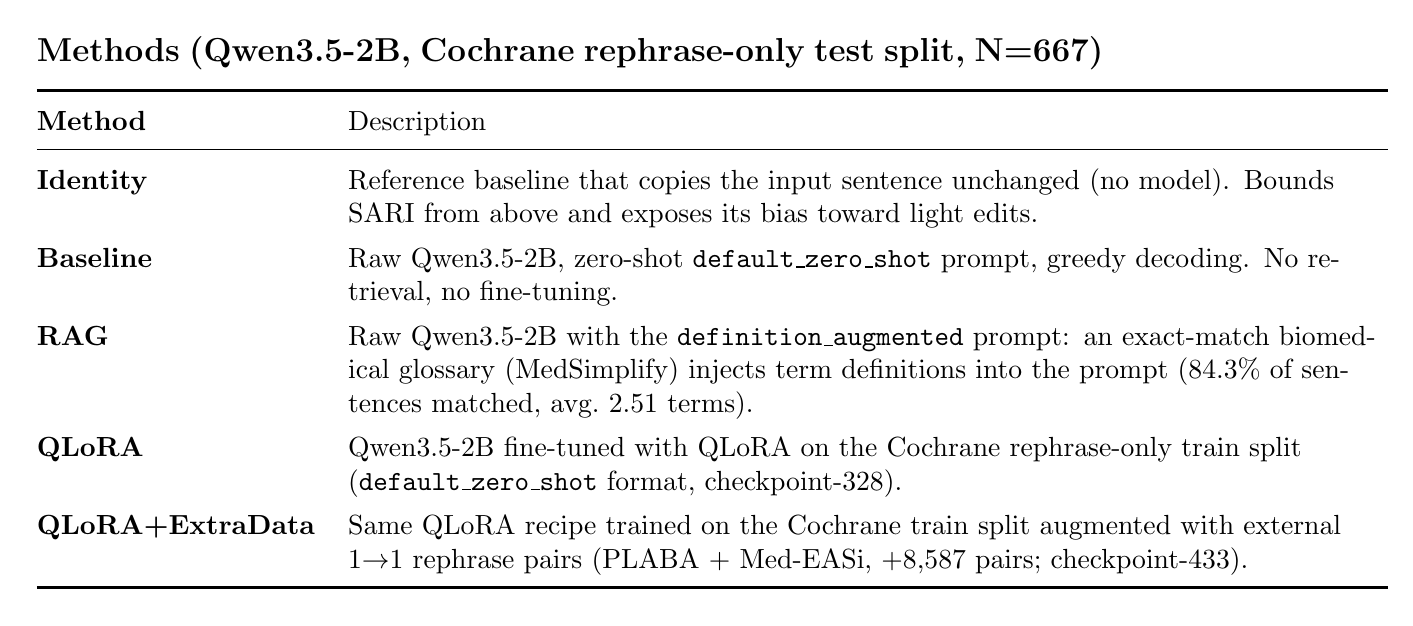
\begin{tikzpicture}
  \node[anchor=north west, align=left, text width=17cm] {%
    {\large\bfseries Methods (Qwen3.5-2B, Cochrane rephrase-only test split, N=667)}\\[6pt]
    \renewcommand{\arraystretch}{1.35}%
    \begin{tabular}{@{}>{\bfseries}l p{13.2cm}@{}}
      \toprule
      Method & Description \\
      \midrule
      Identity &
        Reference baseline that copies the input sentence unchanged (no model).
        Bounds SARI from above and exposes its bias toward light edits. \\
      Baseline &
        Raw Qwen3.5-2B, zero-shot \texttt{default\_zero\_shot} prompt, greedy
        decoding. No retrieval, no fine-tuning. \\
      RAG &
        Raw Qwen3.5-2B with the \texttt{definition\_augmented} prompt: an
        exact-match biomedical glossary (MedSimplify) injects term definitions
        into the prompt (84.3\% of sentences matched, avg.\ 2.51 terms). \\
      QLoRA &
        Qwen3.5-2B fine-tuned with QLoRA on the Cochrane rephrase-only train
        split (\texttt{default\_zero\_shot} format, checkpoint-328). \\
      QLoRA+ExtraData &
        Same QLoRA recipe trained on the Cochrane train split augmented with
        external 1$\to$1 rephrase pairs (PLABA + Med-EASi, +8{,}587 pairs;
        checkpoint-433). \\
      \bottomrule
    \end{tabular}%
  };
\end{tikzpicture}

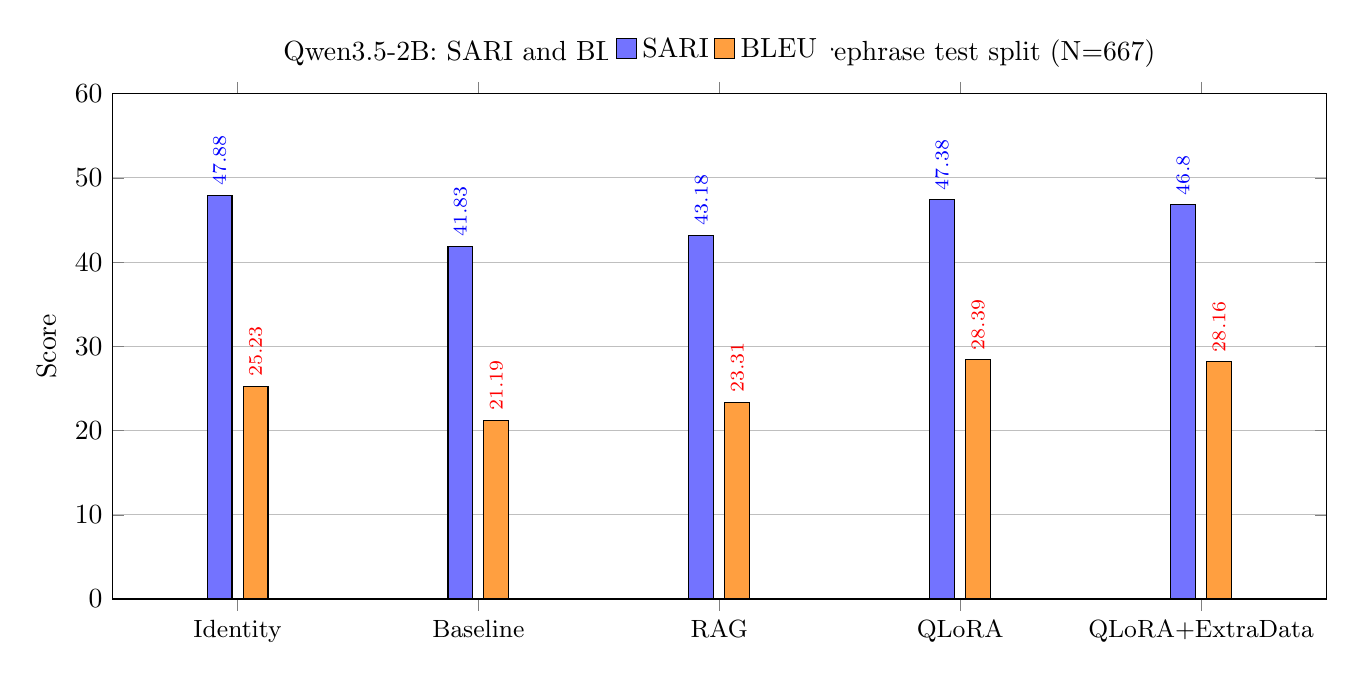
\begin{tikzpicture}
  \begin{axis}[
      width=17cm, height=8cm,
      ybar=4pt,
      bar width=9pt,
      enlarge x limits=0.13,
      ymin=0, ymax=60,
      ymajorgrids=true,
      ylabel={Score},
      symbolic x coords={Identity, Baseline, RAG, QLoRA, QLoRA+ExtraData},
      xtick=data,
      x tick label style={font=\small},
      nodes near coords,
      nodes near coords style={font=\scriptsize, /pgf/number format/fixed, /pgf/number format/precision=2},
      every node near coord/.append style={rotate=90, anchor=west},
      legend style={at={(0.5,1.04)}, anchor=south, legend columns=-1, draw=none},
      legend image code/.code={\draw[#1] (0cm,-0.1cm) rectangle (0.25cm,0.15cm);},
      title={Qwen3.5-2B: SARI and BLEU on Cochrane rephrase test split (N=667)},
    ]
    % SARI
    \addplot+[draw=black, fill=blue!55] coordinates {
      (Identity,47.88) (Baseline,41.83) (RAG,43.18) (QLoRA,47.38) (QLoRA+ExtraData,46.80)
    };
    % BLEU
    \addplot+[draw=black, fill=orange!75] coordinates {
      (Identity,25.23) (Baseline,21.19) (RAG,23.31) (QLoRA,28.39) (QLoRA+ExtraData,28.16)
    };
    \legend{SARI, BLEU}
  \end{axis}
\end{tikzpicture}

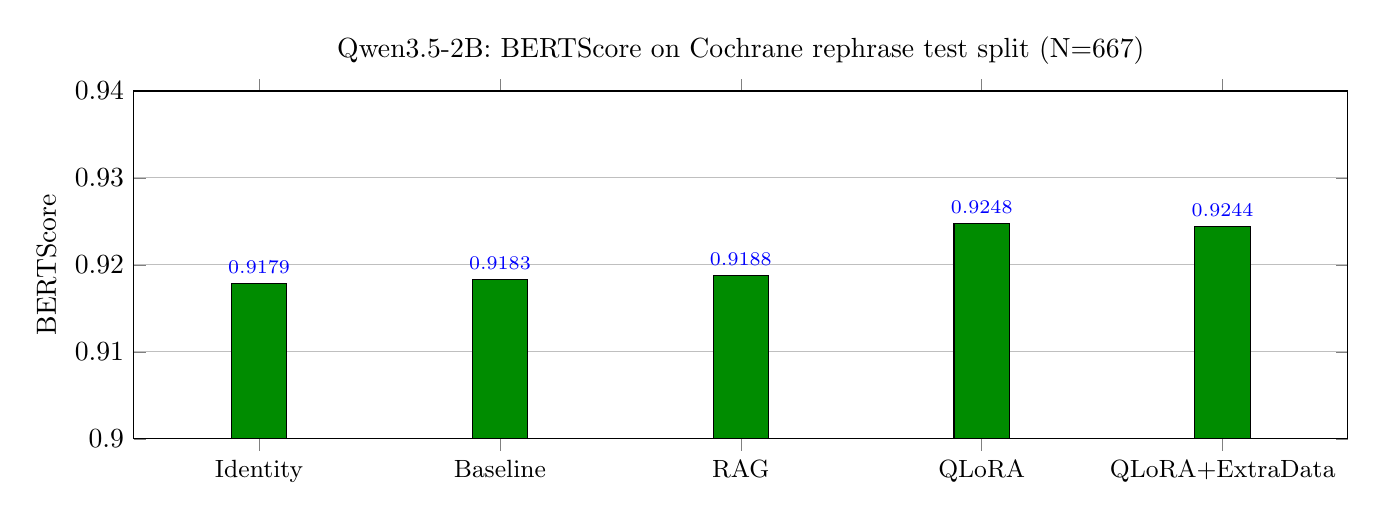
\begin{tikzpicture}
  \begin{axis}[
      width=17cm, height=6cm,
      ybar,
      bar width=20pt,
      enlarge x limits=0.13,
      ymin=0.9, ymax=0.94,
      ymajorgrids=true,
      ylabel={BERTScore},
      symbolic x coords={Identity, Baseline, RAG, QLoRA, QLoRA+ExtraData},
      xtick=data,
      x tick label style={font=\small},
      nodes near coords,
      nodes near coords style={font=\scriptsize, /pgf/number format/fixed, /pgf/number format/precision=4},
      title={Qwen3.5-2B: BERTScore on Cochrane rephrase test split (N=667)},
    ]
    \addplot+[draw=black, fill=green!55!black] coordinates {
      (Identity,0.9179) (Baseline,0.9183) (RAG,0.9188) (QLoRA,0.9248) (QLoRA+ExtraData,0.9244)
    };
  \end{axis}
\end{tikzpicture}
\end{document}
